\documentclass[11pt]{standalone}

\usepackage{ifthen}
\usepackage{amsmath}
\usepackage{tikz} 
\usepackage[d]{esvect}
\usetikzlibrary{shapes.misc}
\usetikzlibrary{arrows,arrows.meta}
\usetikzlibrary{calc,intersections, patterns, math}

\definecolor{pfeil}{RGB}{168,167,167}
\definecolor{salmon}{RGB}{250,128,114}
\definecolor{petrol}{RGB}{0, 118, 136}
\definecolor{darkgoldenrod}{RGB}{184, 134, 11}
\colorlet{petrol-lighter}{petrol!40}
\colorlet{darkgoldenrod-lighter}{darkgoldenrod!40}

\begin{document}

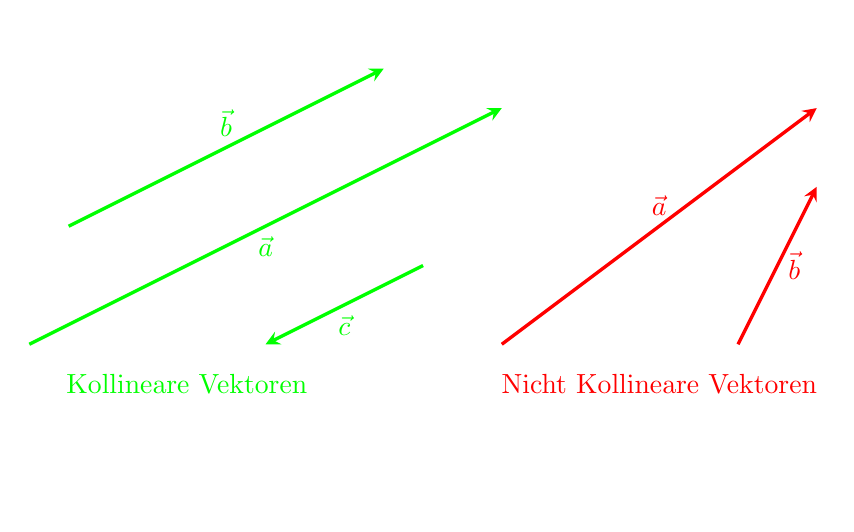
\begin{tikzpicture}[pfeil, >=stealth, very thick]
			
	\draw[transparent] (1,0) rectangle (11,6);
			
			\draw[->, green] (1,2) -- node[below] {$\vec a$} ++ (6,3);
			\draw[->, green] (1.5,3.5) -- node[above] {$\vec b$} ++ (4,2);
			\draw[->, green] (6,3.) -- node[below] {$\vec c$} ++ (-2,-1);
			
			\node[green] at (3,1.5) {Kollineare Vektoren};
			
			\draw[->, red] (7,2) -- node[above] {$\vec a$} ++ (4,3);
			\draw[->, red] (10,2) -- node[right] {$\vec b$} ++ (1,2);
			\node[red] at (9,1.5) {Nicht Kollineare Vektoren};
			
\end{tikzpicture}			

\end{document}
